\documentclass[1p]{elsarticle_modified}
%\bibliographystyle{elsarticle-num}

%\usepackage[colorlinks]{hyperref}
%\usepackage{abbrmath_seonhwa} %\Abb, \Ascr, \Acal ,\Abf, \Afrak
\usepackage{amsfonts}
\usepackage{amssymb}
\usepackage{amsmath}
\usepackage{amsthm}
\usepackage{scalefnt}
\usepackage{amsbsy}
\usepackage{kotex}
\usepackage{caption}
\usepackage{subfig}
\usepackage{color}
\usepackage{graphicx}
\usepackage{xcolor} %% white, black, red, green, blue, cyan, magenta, yellow
\usepackage{float}
\usepackage{setspace}
\usepackage{hyperref}

\usepackage{tikz}
\usetikzlibrary{arrows}

\usepackage{multirow}
\usepackage{array} % fixed length table
\usepackage{hhline}

%%%%%%%%%%%%%%%%%%%%%
\makeatletter
\renewcommand*\env@matrix[1][\arraystretch]{%
	\edef\arraystretch{#1}%
	\hskip -\arraycolsep
	\let\@ifnextchar\new@ifnextchar
	\array{*\c@MaxMatrixCols c}}
\makeatother %https://tex.stackexchange.com/questions/14071/how-can-i-increase-the-line-spacing-in-a-matrix
%%%%%%%%%%%%%%%

\usepackage[normalem]{ulem}

\newcommand{\msout}[1]{\ifmmode\text{\sout{\ensuremath{#1}}}\else\sout{#1}\fi}
%SOURCE: \msout is \stkout macro in https://tex.stackexchange.com/questions/20609/strikeout-in-math-mode

\newcommand{\cancel}[1]{
	\ifmmode
	{\color{red}\msout{#1}}
	\else
	{\color{red}\sout{#1}}
	\fi
}

\newcommand{\add}[1]{
	{\color{blue}\uwave{#1}}
}

\newcommand{\replace}[2]{
	\ifmmode
	{\color{red}\msout{#1}}{\color{blue}\uwave{#2}}
	\else
	{\color{red}\sout{#1}}{\color{blue}\uwave{#2}}
	\fi
}

\newcommand{\Sol}{\mathcal{S}} %segment
\newcommand{\D}{D} %diagram
\newcommand{\A}{\mathcal{A}} %arc


%%%%%%%%%%%%%%%%%%%%%%%%%%%%%5 test

\def\sl{\operatorname{\textup{SL}}(2,\Cbb)}
\def\psl{\operatorname{\textup{PSL}}(2,\Cbb)}
\def\quan{\mkern 1mu \triangleright \mkern 1mu}

\theoremstyle{definition}
\newtheorem{thm}{Theorem}[section]
\newtheorem{prop}[thm]{Proposition}
\newtheorem{lem}[thm]{Lemma}
\newtheorem{ques}[thm]{Question}
\newtheorem{cor}[thm]{Corollary}
\newtheorem{defn}[thm]{Definition}
\newtheorem{exam}[thm]{Example}
\newtheorem{rmk}[thm]{Remark}
\newtheorem{alg}[thm]{Algorithm}

\newcommand{\I}{\sqrt{-1}}
\begin{document}

%\begin{frontmatter}
%
%\title{Boundary parabolic representations of knots up to 8 crossings}
%
%%% Group authors per affiliation:
%\author{Yunhi Cho} 
%\address{Department of Mathematics, University of Seoul, Seoul, Korea}
%\ead{yhcho@uos.ac.kr}
%
%
%\author{Seonhwa Kim} %\fnref{s_kim}}
%\address{Center for Geometry and Physics, Institute for Basic Science, Pohang, 37673, Korea}
%\ead{ryeona17@ibs.re.kr}
%
%\author{Hyuk Kim}
%\address{Department of Mathematical Sciences, Seoul National University, Seoul 08826, Korea}
%\ead{hyukkim@snu.ac.kr}
%
%\author{Seokbeom Yoon}
%\address{Department of Mathematical Sciences, Seoul National University, Seoul, 08826,  Korea}
%\ead{sbyoon15@snu.ac.kr}
%
%\begin{abstract}
%We find all boundary parabolic representation of knots up to 8 crossings.
%
%\end{abstract}
%\begin{keyword}
%    \MSC[2010] 57M25 
%\end{keyword}
%
%\end{frontmatter}

%\linenumbers
%\tableofcontents
%
\newcommand\colored[1]{\textcolor{white}{\rule[-0.35ex]{0.8em}{1.4ex}}\kern-0.8em\color{red} #1}%
%\newcommand\colored[1]{\textcolor{white}{ #1}\kern-2.17ex	\textcolor{white}{ #1}\kern-1.81ex	\textcolor{white}{ #1}\kern-2.15ex\color{red}#1	}

{\Large $\underline{12n_{0473}~(K12n_{0473})}$}

\setlength{\tabcolsep}{10pt}
\renewcommand{\arraystretch}{1.6}
\vspace{1cm}\begin{tabular}{m{100pt}>{\centering\arraybackslash}m{274pt}}
\multirow{5}{120pt}{
	\centering
	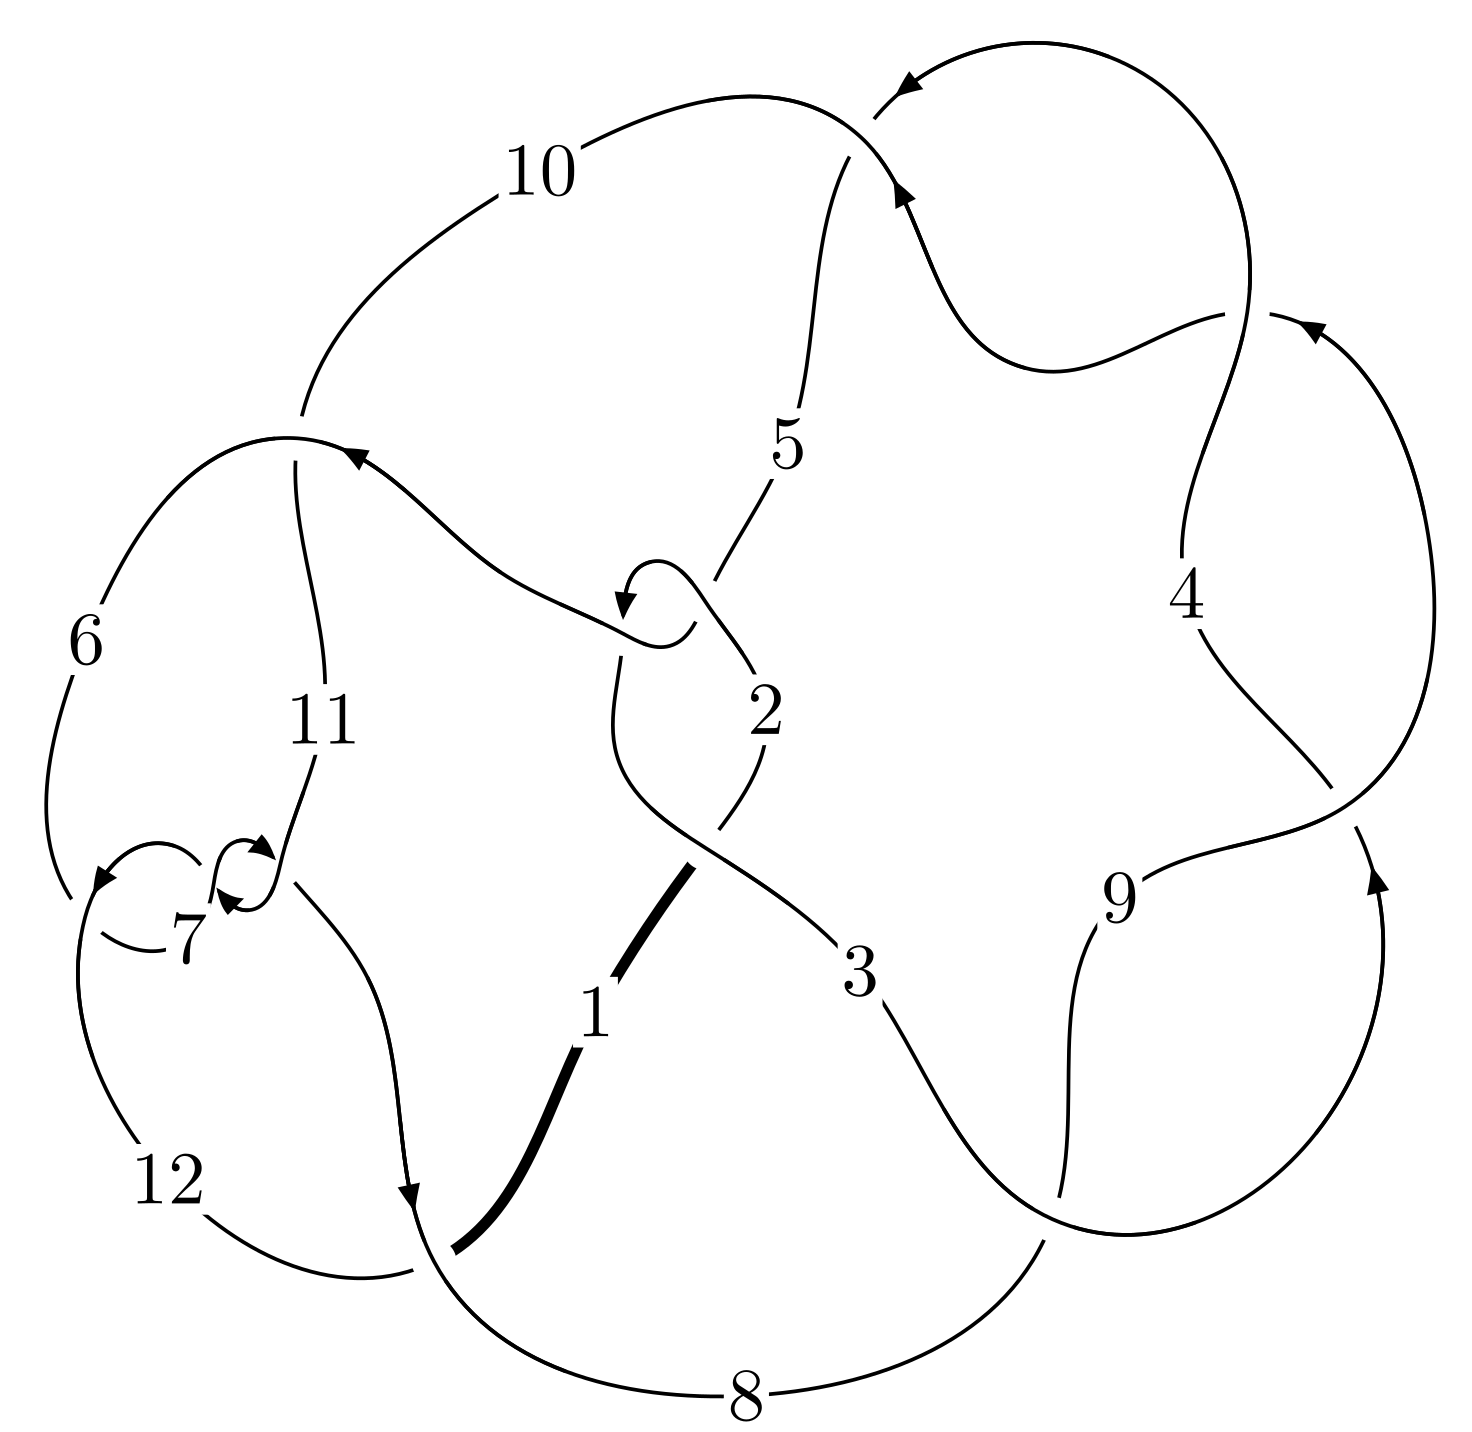
\includegraphics[width=112pt]{../../../GIT/diagram.site/Diagrams/png/2562_12n_0473.png}\\
\ \ \ A knot diagram\footnotemark}&
\allowdisplaybreaks
\textbf{Linearized knot diagam} \\
\cline{2-2}
 &
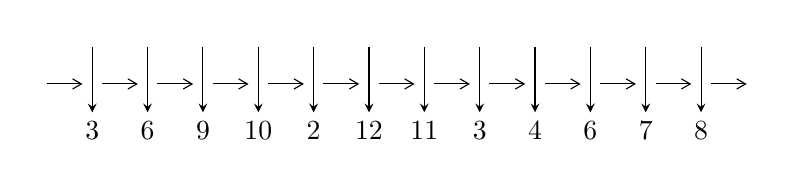
\begin{tikzpicture}[x=20pt, y=17pt]
	% nodes
	\node (C0) at (0, 0) {};
	\node (C1) at (1, 0) {};
	\node (C1U) at (1, +1) {};
	\node (C1D) at (1, -1) {3};

	\node (C2) at (2, 0) {};
	\node (C2U) at (2, +1) {};
	\node (C2D) at (2, -1) {6};

	\node (C3) at (3, 0) {};
	\node (C3U) at (3, +1) {};
	\node (C3D) at (3, -1) {9};

	\node (C4) at (4, 0) {};
	\node (C4U) at (4, +1) {};
	\node (C4D) at (4, -1) {10};

	\node (C5) at (5, 0) {};
	\node (C5U) at (5, +1) {};
	\node (C5D) at (5, -1) {2};

	\node (C6) at (6, 0) {};
	\node (C6U) at (6, +1) {};
	\node (C6D) at (6, -1) {12};

	\node (C7) at (7, 0) {};
	\node (C7U) at (7, +1) {};
	\node (C7D) at (7, -1) {11};

	\node (C8) at (8, 0) {};
	\node (C8U) at (8, +1) {};
	\node (C8D) at (8, -1) {3};

	\node (C9) at (9, 0) {};
	\node (C9U) at (9, +1) {};
	\node (C9D) at (9, -1) {4};

	\node (C10) at (10, 0) {};
	\node (C10U) at (10, +1) {};
	\node (C10D) at (10, -1) {6};

	\node (C11) at (11, 0) {};
	\node (C11U) at (11, +1) {};
	\node (C11D) at (11, -1) {7};

	\node (C12) at (12, 0) {};
	\node (C12U) at (12, +1) {};
	\node (C12D) at (12, -1) {8};
	\node (C13) at (13, 0) {};

	% arrows
	\draw[->,>={angle 60}]
	(C0) edge (C1) (C1) edge (C2) (C2) edge (C3) (C3) edge (C4) (C4) edge (C5) (C5) edge (C6) (C6) edge (C7) (C7) edge (C8) (C8) edge (C9) (C9) edge (C10) (C10) edge (C11) (C11) edge (C12) (C12) edge (C13) ;	\draw[->,>=stealth]
	(C1U) edge (C1D) (C2U) edge (C2D) (C3U) edge (C3D) (C4U) edge (C4D) (C5U) edge (C5D) (C6U) edge (C6D) (C7U) edge (C7D) (C8U) edge (C8D) (C9U) edge (C9D) (C10U) edge (C10D) (C11U) edge (C11D) (C12U) edge (C12D) ;
	\end{tikzpicture} \\
\hhline{~~} \\& 
\textbf{Solving Sequence} \\ \cline{2-2} 
 &
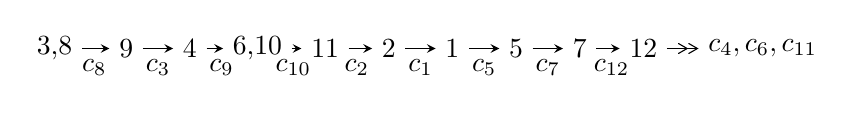
\begin{tikzpicture}[x=23pt, y=7pt]
	% node
	\node (A0) at (-1/8, 0) {3,8};
	\node (A1) at (1, 0) {9};
	\node (A2) at (2, 0) {4};
	\node (A3) at (49/16, 0) {6,10};
	\node (A4) at (33/8, 0) {11};
	\node (A5) at (41/8, 0) {2};
	\node (A6) at (49/8, 0) {1};
	\node (A7) at (57/8, 0) {5};
	\node (A8) at (65/8, 0) {7};
	\node (A9) at (73/8, 0) {12};
	\node (C1) at (1/2, -1) {$c_{8}$};
	\node (C2) at (3/2, -1) {$c_{3}$};
	\node (C3) at (5/2, -1) {$c_{9}$};
	\node (C4) at (29/8, -1) {$c_{10}$};
	\node (C5) at (37/8, -1) {$c_{2}$};
	\node (C6) at (45/8, -1) {$c_{1}$};
	\node (C7) at (53/8, -1) {$c_{5}$};
	\node (C8) at (61/8, -1) {$c_{7}$};
	\node (C9) at (69/8, -1) {$c_{12}$};
	\node (A10) at (11, 0) {$c_{4},c_{6},c_{11}$};

	% edge
	\draw[->,>=stealth]	
	(A0) edge (A1) (A1) edge (A2) (A2) edge (A3) (A3) edge (A4) (A4) edge (A5) (A5) edge (A6) (A6) edge (A7) (A7) edge (A8) (A8) edge (A9) ;
	\draw[->>,>={angle 60}]	
	(A9) edge (A10);
\end{tikzpicture} \\ 

\end{tabular} \\

\footnotetext{
The image of knot diagram is generated by the software ``\textbf{Draw programme}" developed by Andrew Bartholomew(\url{http://www.layer8.co.uk/maths/draw/index.htm\#Running-draw}), where we modified some parts for our purpose(\url{https://github.com/CATsTAILs/LinksPainter}).
}\phantom \\ \newline 
\centering \textbf{Ideals for irreducible components\footnotemark of $X_{\text{par}}$} 
 
\begin{align*}
I^u_{1}&=\langle 
5447 u^8-4753 u^7+\cdots+46532 b+23300,\;-461 u^8-3128 u^7+\cdots+93064 a-27096,\\
\phantom{I^u_{1}}&\phantom{= \langle  }u^9-18 u^7-36 u^6+12 u^5+68 u^4+36 u^3+8 u^2+24 u+8\rangle \\
I^u_{2}&=\langle 
b^3- b^2+1,\;2 a- u,\;u^2-2\rangle \\
\\
I^v_{1}&=\langle 
a,\;v^2+b-1,\;v^3- v+1\rangle \\
\end{align*}
\raggedright * 3 irreducible components of $\dim_{\mathbb{C}}=0$, with total 18 representations.\\
\footnotetext{All coefficients of polynomials are rational numbers. But the coefficients are sometimes approximated in decimal forms when there is not enough margin.}
\newpage
\renewcommand{\arraystretch}{1}
\centering \section*{I. $I^u_{1}= \langle 5447 u^8-4753 u^7+\cdots+46532 b+23300,\;-461 u^8-3128 u^7+\cdots+93064 a-27096,\;u^9-18 u^7+\cdots+24 u+8 \rangle$}
\flushleft \textbf{(i) Arc colorings}\\
\begin{tabular}{m{7pt} m{180pt} m{7pt} m{180pt} }
\flushright $a_{3}=$&$\begin{pmatrix}0\\u\end{pmatrix}$ \\
\flushright $a_{8}=$&$\begin{pmatrix}1\\0\end{pmatrix}$ \\
\flushright $a_{9}=$&$\begin{pmatrix}1\\u^2\end{pmatrix}$ \\
\flushright $a_{4}=$&$\begin{pmatrix}- u\\- u^3+u\end{pmatrix}$ \\
\flushright $a_{6}=$&$\begin{pmatrix}0.00495358 u^{8}+0.0336113 u^{7}+\cdots-1.27001 u+0.291154\\-0.117059 u^{8}+0.102145 u^{7}+\cdots-0.727843 u-0.500731\end{pmatrix}$ \\
\flushright $a_{10}=$&$\begin{pmatrix}- u^2+1\\- u^4+2 u^2\end{pmatrix}$ \\
\flushright $a_{11}=$&$\begin{pmatrix}0.0289801 u^{8}-0.0392633 u^{7}+\cdots-0.182670 u+0.813977\\0.0609903 u^{8}-0.0503739 u^{7}+\cdots+1.76017 u+0.788705\end{pmatrix}$ \\
\flushright $a_{2}=$&$\begin{pmatrix}0.0267235 u^{8}-0.0442706 u^{7}+\cdots+0.191954 u-0.199347\\0.0998238 u^{8}-0.159439 u^{7}+\cdots+1.80830 u+0.494198\end{pmatrix}$ \\
\flushright $a_{1}=$&$\begin{pmatrix}0.0267235 u^{8}-0.0442706 u^{7}+\cdots+0.191954 u-0.199347\\0.00758618 u^{8}-0.00221353 u^{7}+\cdots+0.959598 u+0.140033\end{pmatrix}$ \\
\flushright $a_{5}=$&$\begin{pmatrix}u^3-2 u\\u^5-3 u^3+u\end{pmatrix}$ \\
\flushright $a_{7}=$&$\begin{pmatrix}0.0326442 u^{8}-0.0442276 u^{7}+\cdots-0.952893 u+0.526090\\-0.0316341 u^{8}-0.0297215 u^{7}+\cdots-0.338606 u-0.139173\end{pmatrix}$ \\
\flushright $a_{12}=$&$\begin{pmatrix}0.0343097 u^{8}-0.0464841 u^{7}+\cdots+1.15155 u-0.0593140\\0.00758618 u^{8}-0.00221353 u^{7}+\cdots+0.959598 u+0.140033\end{pmatrix}$\\&\end{tabular}
\flushleft \textbf{(ii) Obstruction class $= -1$}\\~\\
\flushleft \textbf{(iii) Cusp Shapes $= -\frac{20957}{46532} u^8+\frac{5941}{23266} u^7+\frac{185067}{23266} u^6+\frac{274717}{23266} u^5-\frac{139019}{11633} u^4-\frac{299261}{11633} u^3-\frac{57101}{11633} u^2+\frac{28694}{11633} u-\frac{223158}{11633}$}\\~\\
\newpage\renewcommand{\arraystretch}{1}
\flushleft \textbf{(iv) u-Polynomials at the component}\newline \\
\begin{tabular}{m{50pt}|m{274pt}}
Crossings & \hspace{64pt}u-Polynomials at each crossing \\
\hline $$\begin{aligned}c_{1}\end{aligned}$$&$\begin{aligned}
&u^9+73 u^8+\cdots+729 u+49
\end{aligned}$\\
\hline $$\begin{aligned}c_{2},c_{5}\end{aligned}$$&$\begin{aligned}
&u^9+13 u^8+48 u^7+72 u^6+18 u^5-14 u^4-40 u^3-27 u-7
\end{aligned}$\\
\hline $$\begin{aligned}c_{3},c_{4},c_{8}\\c_{9}\end{aligned}$$&$\begin{aligned}
&u^9-18 u^7-36 u^6+12 u^5+68 u^4+36 u^3+8 u^2+24 u+8
\end{aligned}$\\
\hline $$\begin{aligned}c_{6},c_{7},c_{11}\end{aligned}$$&$\begin{aligned}
&u^9+3 u^8+7 u^7+14 u^6+14 u^5+25 u^4+11 u^3+15 u^2-1
\end{aligned}$\\
\hline $$\begin{aligned}c_{10},c_{12}\end{aligned}$$&$\begin{aligned}
&u^9+9 u^8-73 u^7+56 u^6+430 u^5-75 u^4-417 u^3+173 u^2+36 u-13
\end{aligned}$\\
\hline
\end{tabular}\\~\\
\newpage\renewcommand{\arraystretch}{1}
\flushleft \textbf{(v) Riley Polynomials at the component}\newline \\
\begin{tabular}{m{50pt}|m{274pt}}
Crossings & \hspace{64pt}Riley Polynomials at each crossing \\
\hline $$\begin{aligned}c_{1}\end{aligned}$$&$\begin{aligned}
&y^9-4393 y^8+\cdots+723913 y-2401
\end{aligned}$\\
\hline $$\begin{aligned}c_{2},c_{5}\end{aligned}$$&$\begin{aligned}
&y^9-73 y^8+\cdots+729 y-49
\end{aligned}$\\
\hline $$\begin{aligned}c_{3},c_{4},c_{8}\\c_{9}\end{aligned}$$&$\begin{aligned}
&y^9-36 y^8+\cdots+448 y-64
\end{aligned}$\\
\hline $$\begin{aligned}c_{6},c_{7},c_{11}\end{aligned}$$&$\begin{aligned}
&y^9+5 y^8-7 y^7-128 y^6-440 y^5-731 y^4-601 y^3-175 y^2+30 y-1
\end{aligned}$\\
\hline $$\begin{aligned}c_{10},c_{12}\end{aligned}$$&$\begin{aligned}
&y^9-227 y^8+\cdots+5794 y-169
\end{aligned}$\\
\hline
\end{tabular}\\~\\
\newpage\flushleft \textbf{(vi) Complex Volumes and Cusp Shapes}
$$\begin{array}{c|c|c}  
\text{Solutions to }I^u_{1}& \I (\text{vol} + \sqrt{-1}CS) & \text{Cusp shape}\\
 \hline 
\begin{aligned}
u &= -1.186450 + 0.424170 I \\
a &= \phantom{-}0.251161 + 0.846300 I \\
b &= \phantom{-}1.76218 + 0.93575 I\end{aligned}
 & -1.02910 - 2.89378 I & -13.46616 + 2.37667 I \\ \hline\begin{aligned}
u &= -1.186450 - 0.424170 I \\
a &= \phantom{-}0.251161 - 0.846300 I \\
b &= \phantom{-}1.76218 - 0.93575 I\end{aligned}
 & -1.02910 + 2.89378 I & -13.46616 - 2.37667 I \\ \hline\begin{aligned}
u &= \phantom{-}0.273011 + 0.580428 I \\
a &= -0.750166 - 0.744053 I \\
b &= \phantom{-}1.201410 + 0.238186 I\end{aligned}
 & \phantom{-}2.44926 - 1.76826 I & -8.73509 + 3.07632 I \\ \hline\begin{aligned}
u &= \phantom{-}0.273011 - 0.580428 I \\
a &= -0.750166 + 0.744053 I \\
b &= \phantom{-}1.201410 - 0.238186 I\end{aligned}
 & \phantom{-}2.44926 + 1.76826 I & -8.73509 - 3.07632 I \\ \hline\begin{aligned}
u &= \phantom{-}1.44806\phantom{ +0.000000I} \\
a &= \phantom{-}0.605279\phantom{ +0.000000I} \\
b &= -0.107770\phantom{ +0.000000I}\end{aligned}
 & -6.65928\phantom{ +0.000000I} & -13.3420\phantom{ +0.000000I} \\ \hline\begin{aligned}
u &= -0.347212\phantom{ +0.000000I} \\
a &= \phantom{-}0.692622\phantom{ +0.000000I} \\
b &= -0.151972\phantom{ +0.000000I}\end{aligned}
 & -0.501693\phantom{ +0.000000I} & -19.7740\phantom{ +0.000000I} \\ \hline\begin{aligned}
u &= -2.09595 + 0.74847 I \\
a &= \phantom{-}1.180400 - 0.226493 I \\
b &= \phantom{-}1.57561 - 4.87250 I\end{aligned}
 & \phantom{-}13.5998 + 8.3082 I & -13.79311 - 2.86755 I \\ \hline\begin{aligned}
u &= -2.09595 - 0.74847 I \\
a &= \phantom{-}1.180400 + 0.226493 I \\
b &= \phantom{-}1.57561 + 4.87250 I\end{aligned}
 & \phantom{-}13.5998 - 8.3082 I & -13.79311 + 2.86755 I \\ \hline\begin{aligned}
u &= \phantom{-}4.91794\phantom{ +0.000000I} \\
a &= -1.66068\phantom{ +0.000000I} \\
b &= -37.8186\phantom{ +0.000000I}\end{aligned}
 & \phantom{-}6.72995\phantom{ +0.000000I} & -14.8960\phantom{ +0.000000I}\\
 \hline 
 \end{array}$$\newpage\newpage\renewcommand{\arraystretch}{1}
\centering \section*{II. $I^u_{2}= \langle b^3- b^2+1,\;2 a- u,\;u^2-2 \rangle$}
\flushleft \textbf{(i) Arc colorings}\\
\begin{tabular}{m{7pt} m{180pt} m{7pt} m{180pt} }
\flushright $a_{3}=$&$\begin{pmatrix}0\\u\end{pmatrix}$ \\
\flushright $a_{8}=$&$\begin{pmatrix}1\\0\end{pmatrix}$ \\
\flushright $a_{9}=$&$\begin{pmatrix}1\\2\end{pmatrix}$ \\
\flushright $a_{4}=$&$\begin{pmatrix}- u\\- u\end{pmatrix}$ \\
\flushright $a_{6}=$&$\begin{pmatrix}\frac{1}{2} u\\b\end{pmatrix}$ \\
\flushright $a_{10}=$&$\begin{pmatrix}-1\\0\end{pmatrix}$ \\
\flushright $a_{11}=$&$\begin{pmatrix}-\frac{1}{2} b u-1\\- b^2\end{pmatrix}$ \\
\flushright $a_{2}=$&$\begin{pmatrix}\frac{1}{2} u\\b+u\end{pmatrix}$ \\
\flushright $a_{1}=$&$\begin{pmatrix}\frac{1}{2} u\\b\end{pmatrix}$ \\
\flushright $a_{5}=$&$\begin{pmatrix}0\\- u\end{pmatrix}$ \\
\flushright $a_{7}=$&$\begin{pmatrix}-\frac{1}{2} b^2 u- b^2+\frac{1}{2} u+1\\- b^2+b+1\end{pmatrix}$ \\
\flushright $a_{12}=$&$\begin{pmatrix}b+\frac{1}{2} u\\b\end{pmatrix}$\\&\end{tabular}
\flushleft \textbf{(ii) Obstruction class $= 1$}\\~\\
\flushleft \textbf{(iii) Cusp Shapes $= 4 b-20$}\\~\\
\newpage\renewcommand{\arraystretch}{1}
\flushleft \textbf{(iv) u-Polynomials at the component}\newline \\
\begin{tabular}{m{50pt}|m{274pt}}
Crossings & \hspace{64pt}u-Polynomials at each crossing \\
\hline $$\begin{aligned}c_{1},c_{5}\end{aligned}$$&$\begin{aligned}
&(u-1)^6
\end{aligned}$\\
\hline $$\begin{aligned}c_{2}\end{aligned}$$&$\begin{aligned}
&(u+1)^6
\end{aligned}$\\
\hline $$\begin{aligned}c_{3},c_{4},c_{8}\\c_{9}\end{aligned}$$&$\begin{aligned}
&(u^2-2)^3
\end{aligned}$\\
\hline $$\begin{aligned}c_{6},c_{7}\end{aligned}$$&$\begin{aligned}
&(u^3+u^2+2 u+1)^2
\end{aligned}$\\
\hline $$\begin{aligned}c_{10},c_{12}\end{aligned}$$&$\begin{aligned}
&(u^3+u^2-1)^2
\end{aligned}$\\
\hline $$\begin{aligned}c_{11}\end{aligned}$$&$\begin{aligned}
&(u^3- u^2+2 u-1)^2
\end{aligned}$\\
\hline
\end{tabular}\\~\\
\newpage\renewcommand{\arraystretch}{1}
\flushleft \textbf{(v) Riley Polynomials at the component}\newline \\
\begin{tabular}{m{50pt}|m{274pt}}
Crossings & \hspace{64pt}Riley Polynomials at each crossing \\
\hline $$\begin{aligned}c_{1},c_{2},c_{5}\end{aligned}$$&$\begin{aligned}
&(y-1)^6
\end{aligned}$\\
\hline $$\begin{aligned}c_{3},c_{4},c_{8}\\c_{9}\end{aligned}$$&$\begin{aligned}
&(y-2)^6
\end{aligned}$\\
\hline $$\begin{aligned}c_{6},c_{7},c_{11}\end{aligned}$$&$\begin{aligned}
&(y^3+3 y^2+2 y-1)^2
\end{aligned}$\\
\hline $$\begin{aligned}c_{10},c_{12}\end{aligned}$$&$\begin{aligned}
&(y^3- y^2+2 y-1)^2
\end{aligned}$\\
\hline
\end{tabular}\\~\\
\newpage\flushleft \textbf{(vi) Complex Volumes and Cusp Shapes}
$$\begin{array}{c|c|c}  
\text{Solutions to }I^u_{2}& \I (\text{vol} + \sqrt{-1}CS) & \text{Cusp shape}\\
 \hline 
\begin{aligned}
u &= \phantom{-}1.41421\phantom{ +0.000000I} \\
a &= \phantom{-}0.707107\phantom{ +0.000000I} \\
b &= \phantom{-}0.877439 + 0.744862 I\end{aligned}
 & -3.55561 - 2.82812 I & -16.4902 + 2.9794 I \\ \hline\begin{aligned}
u &= \phantom{-}1.41421\phantom{ +0.000000I} \\
a &= \phantom{-}0.707107\phantom{ +0.000000I} \\
b &= \phantom{-}0.877439 - 0.744862 I\end{aligned}
 & -3.55561 + 2.82812 I & -16.4902 - 2.9794 I \\ \hline\begin{aligned}
u &= \phantom{-}1.41421\phantom{ +0.000000I} \\
a &= \phantom{-}0.707107\phantom{ +0.000000I} \\
b &= -0.754878\phantom{ +0.000000I}\end{aligned}
 & -7.69319\phantom{ +0.000000I} & -23.0200\phantom{ +0.000000I} \\ \hline\begin{aligned}
u &= -1.41421\phantom{ +0.000000I} \\
a &= -0.707107\phantom{ +0.000000I} \\
b &= \phantom{-}0.877439 + 0.744862 I\end{aligned}
 & -3.55561 - 2.82812 I & -16.4902 + 2.9794 I \\ \hline\begin{aligned}
u &= -1.41421\phantom{ +0.000000I} \\
a &= -0.707107\phantom{ +0.000000I} \\
b &= \phantom{-}0.877439 - 0.744862 I\end{aligned}
 & -3.55561 + 2.82812 I & -16.4902 - 2.9794 I \\ \hline\begin{aligned}
u &= -1.41421\phantom{ +0.000000I} \\
a &= -0.707107\phantom{ +0.000000I} \\
b &= -0.754878\phantom{ +0.000000I}\end{aligned}
 & -7.69319\phantom{ +0.000000I} & -23.0200\phantom{ +0.000000I}\\
 \hline 
 \end{array}$$\newpage\newpage\renewcommand{\arraystretch}{1}
\centering \section*{III. $I^v_{1}= \langle a,\;v^2+b-1,\;v^3- v+1 \rangle$}
\flushleft \textbf{(i) Arc colorings}\\
\begin{tabular}{m{7pt} m{180pt} m{7pt} m{180pt} }
\flushright $a_{3}=$&$\begin{pmatrix}v\\0\end{pmatrix}$ \\
\flushright $a_{8}=$&$\begin{pmatrix}1\\0\end{pmatrix}$ \\
\flushright $a_{9}=$&$\begin{pmatrix}1\\0\end{pmatrix}$ \\
\flushright $a_{4}=$&$\begin{pmatrix}v\\0\end{pmatrix}$ \\
\flushright $a_{6}=$&$\begin{pmatrix}0\\- v^2+1\end{pmatrix}$ \\
\flushright $a_{10}=$&$\begin{pmatrix}1\\0\end{pmatrix}$ \\
\flushright $a_{11}=$&$\begin{pmatrix}1\\- v^2- v+1\end{pmatrix}$ \\
\flushright $a_{2}=$&$\begin{pmatrix}v\\v^2-1\end{pmatrix}$ \\
\flushright $a_{1}=$&$\begin{pmatrix}0\\v^2-1\end{pmatrix}$ \\
\flushright $a_{5}=$&$\begin{pmatrix}v\\0\end{pmatrix}$ \\
\flushright $a_{7}=$&$\begin{pmatrix}v^2+v\\v+1\end{pmatrix}$ \\
\flushright $a_{12}=$&$\begin{pmatrix}v^2-1\\v^2-1\end{pmatrix}$\\&\end{tabular}
\flushleft \textbf{(ii) Obstruction class $= 1$}\\~\\
\flushleft \textbf{(iii) Cusp Shapes $= -4 v^2-2 v-10$}\\~\\
\newpage\renewcommand{\arraystretch}{1}
\flushleft \textbf{(iv) u-Polynomials at the component}\newline \\
\begin{tabular}{m{50pt}|m{274pt}}
Crossings & \hspace{64pt}u-Polynomials at each crossing \\
\hline $$\begin{aligned}c_{1},c_{2}\end{aligned}$$&$\begin{aligned}
&(u-1)^3
\end{aligned}$\\
\hline $$\begin{aligned}c_{3},c_{4},c_{8}\\c_{9}\end{aligned}$$&$\begin{aligned}
&u^3
\end{aligned}$\\
\hline $$\begin{aligned}c_{5}\end{aligned}$$&$\begin{aligned}
&(u+1)^3
\end{aligned}$\\
\hline $$\begin{aligned}c_{6},c_{7}\end{aligned}$$&$\begin{aligned}
&u^3- u^2+2 u-1
\end{aligned}$\\
\hline $$\begin{aligned}c_{10},c_{12}\end{aligned}$$&$\begin{aligned}
&u^3- u^2+1
\end{aligned}$\\
\hline $$\begin{aligned}c_{11}\end{aligned}$$&$\begin{aligned}
&u^3+u^2+2 u+1
\end{aligned}$\\
\hline
\end{tabular}\\~\\
\newpage\renewcommand{\arraystretch}{1}
\flushleft \textbf{(v) Riley Polynomials at the component}\newline \\
\begin{tabular}{m{50pt}|m{274pt}}
Crossings & \hspace{64pt}Riley Polynomials at each crossing \\
\hline $$\begin{aligned}c_{1},c_{2},c_{5}\end{aligned}$$&$\begin{aligned}
&(y-1)^3
\end{aligned}$\\
\hline $$\begin{aligned}c_{3},c_{4},c_{8}\\c_{9}\end{aligned}$$&$\begin{aligned}
&y^3
\end{aligned}$\\
\hline $$\begin{aligned}c_{6},c_{7},c_{11}\end{aligned}$$&$\begin{aligned}
&y^3+3 y^2+2 y-1
\end{aligned}$\\
\hline $$\begin{aligned}c_{10},c_{12}\end{aligned}$$&$\begin{aligned}
&y^3- y^2+2 y-1
\end{aligned}$\\
\hline
\end{tabular}\\~\\
\newpage\flushleft \textbf{(vi) Complex Volumes and Cusp Shapes}
$$\begin{array}{c|c|c}  
\text{Solutions to }I^v_{1}& \I (\text{vol} + \sqrt{-1}CS) & \text{Cusp shape}\\
 \hline 
\begin{aligned}
v &= \phantom{-}0.662359 + 0.562280 I \\
a &= \phantom{-0.000000 } 0 \\
b &= \phantom{-}0.877439 - 0.744862 I\end{aligned}
 & \phantom{-}1.37919 + 2.82812 I & -11.81496 - 4.10401 I \\ \hline\begin{aligned}
v &= \phantom{-}0.662359 - 0.562280 I \\
a &= \phantom{-0.000000 } 0 \\
b &= \phantom{-}0.877439 + 0.744862 I\end{aligned}
 & \phantom{-}1.37919 - 2.82812 I & -11.81496 + 4.10401 I \\ \hline\begin{aligned}
v &= -1.32472\phantom{ +0.000000I} \\
a &= \phantom{-0.000000 } 0 \\
b &= -0.754878\phantom{ +0.000000I}\end{aligned}
 & -2.75839\phantom{ +0.000000I} & -14.3700\phantom{ +0.000000I}\\
 \hline 
 \end{array}$$\newpage
\newpage\renewcommand{\arraystretch}{1}
\centering \section*{ IV. u-Polynomials}
\begin{tabular}{m{50pt}|m{274pt}}
Crossings & \hspace{64pt}u-Polynomials at each crossing \\
\hline $$\begin{aligned}c_{1}\end{aligned}$$&$\begin{aligned}
&((u-1)^9)(u^9+73 u^8+\cdots+729 u+49)
\end{aligned}$\\
\hline $$\begin{aligned}c_{2}\end{aligned}$$&$\begin{aligned}
&(u-1)^3(u+1)^6\\
&\cdot(u^9+13 u^8+48 u^7+72 u^6+18 u^5-14 u^4-40 u^3-27 u-7)
\end{aligned}$\\
\hline $$\begin{aligned}c_{3},c_{4},c_{8}\\c_{9}\end{aligned}$$&$\begin{aligned}
&u^3(u^2-2)^3(u^9-18 u^7+\cdots+24 u+8)
\end{aligned}$\\
\hline $$\begin{aligned}c_{5}\end{aligned}$$&$\begin{aligned}
&(u-1)^6(u+1)^3\\
&\cdot(u^9+13 u^8+48 u^7+72 u^6+18 u^5-14 u^4-40 u^3-27 u-7)
\end{aligned}$\\
\hline $$\begin{aligned}c_{6},c_{7}\end{aligned}$$&$\begin{aligned}
&(u^3- u^2+2 u-1)(u^3+u^2+2 u+1)^2\\
&\cdot(u^9+3 u^8+7 u^7+14 u^6+14 u^5+25 u^4+11 u^3+15 u^2-1)
\end{aligned}$\\
\hline $$\begin{aligned}c_{10},c_{12}\end{aligned}$$&$\begin{aligned}
&(u^3- u^2+1)(u^3+u^2-1)^2\\
&\cdot(u^9+9 u^8-73 u^7+56 u^6+430 u^5-75 u^4-417 u^3+173 u^2+36 u-13)
\end{aligned}$\\
\hline $$\begin{aligned}c_{11}\end{aligned}$$&$\begin{aligned}
&(u^3- u^2+2 u-1)^2(u^3+u^2+2 u+1)\\
&\cdot(u^9+3 u^8+7 u^7+14 u^6+14 u^5+25 u^4+11 u^3+15 u^2-1)
\end{aligned}$\\
\hline
\end{tabular}\newpage\renewcommand{\arraystretch}{1}
\centering \section*{ V. Riley Polynomials}
\begin{tabular}{m{50pt}|m{274pt}}
Crossings & \hspace{64pt}Riley Polynomials at each crossing \\
\hline $$\begin{aligned}c_{1}\end{aligned}$$&$\begin{aligned}
&((y-1)^9)(y^9-4393 y^8+\cdots+723913 y-2401)
\end{aligned}$\\
\hline $$\begin{aligned}c_{2},c_{5}\end{aligned}$$&$\begin{aligned}
&((y-1)^9)(y^9-73 y^8+\cdots+729 y-49)
\end{aligned}$\\
\hline $$\begin{aligned}c_{3},c_{4},c_{8}\\c_{9}\end{aligned}$$&$\begin{aligned}
&y^3(y-2)^6(y^{9}-36 y^{8}+\cdots+448 y-64)
\end{aligned}$\\
\hline $$\begin{aligned}c_{6},c_{7},c_{11}\end{aligned}$$&$\begin{aligned}
&(y^3+3 y^2+2 y-1)^3\\
&\cdot(y^9+5 y^8-7 y^7-128 y^6-440 y^5-731 y^4-601 y^3-175 y^2+30 y-1)
\end{aligned}$\\
\hline $$\begin{aligned}c_{10},c_{12}\end{aligned}$$&$\begin{aligned}
&((y^3- y^2+2 y-1)^3)(y^9-227 y^8+\cdots+5794 y-169)
\end{aligned}$\\
\hline
\end{tabular}
\vskip 2pc
\end{document}